\documentclass{beamer}
\usepackage{sdp}

\title{Дървета за търсене}

\date{11 декември 2015 г.}

\titlegraphic{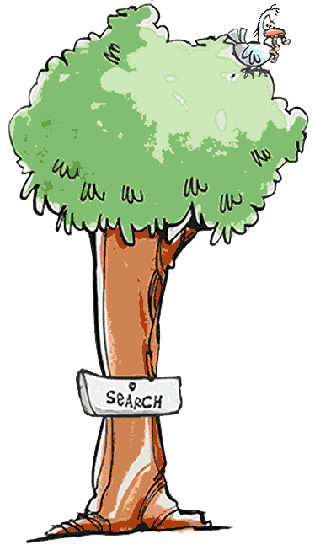
\includegraphics[height=0.35\textheight]{images/searchtree.png}}

\forestset{default/.style={baseline,for tree={fill=diagramblue,draw,circle,inner
      sep=0pt,minimum size=4ex,edge=->}}}

\forestset{scheme/.style=default,for tree={minimum size=6ex}}

\forestset{tri/.style={shape=isosceles triangle,shape border rotate=90,minimum height=6em,child anchor=north,anchor=north}}

\forestset{trismall/.style={tri,minimum height=4em}}

\forestset{remove/.style={tikz={\draw[thick,red] (!.north west) -- (!.south east); \draw[thick,red] (!.north east) -- (!.south west);}}}

\forestset{removesmall/.style={tikz={\draw[thick,red] (!.north west)++(1.5ex,1.5ex) -- ++(3ex,-3ex); \draw[thick,red] (!.north west)++(4.5ex,1.5ex) -- ++(-3ex,-3ex); \node at (!.north west) [xshift=3ex,circle,draw,inner sep=0.2ex]{Y};}}}

\newcommand{\samplebinordtree}{%
  \begin{forest}
    default [5 [3 [2 [1] [,phantom]] [4]] [8 [6 [,phantom] [7] ] [10]]]
  \end{forest}%
}

\begin{document}

\begin{frame}
  \titlepage
\end{frame}

\begin{frame}
  \frametitle{Дървета за търсене}
  \begin{itemize}
  \item Организация, която позволява бързо намиране на елементи в дървото
  \item Разчита на \textbf{линейна наредба} на елементите
  \item Основни операции:
    \begin{itemize}
    \item \tt{create()} --- създаване на празно дърво за търсене
    \item \tt{insert(x)} --- включване на елемент
    \item \tt{remove(x)} --- изключване на елемент
    \item \tt{search(x)} --- търсене на елемент
    \end{itemize}
  \item Обикновено елементите са двойки (ключ,стойност)
  \item Елементите са наредени относно ключовете си
  \item Стойностите носят данните на елемента
  \end{itemize}
\end{frame}

\section{Двоично дърво за търсене}

\begin{frame}
  \frametitle{Двоично дърво за търсене}
  \begin{definition}[Двоично дърво за търсене]
    \begin{itemize}
    \item Празното дърво $\bot$ е ДДТ
    \item $(X,L,R)$ е ДДТ, ако
      \begin{itemize}
      \item $X$ е по-голямо от от всички елементи в $L$
      \item $X$ е по-малко от от всички елементи в $R$
      \item $L$ и $R$ също са ДДТ
      \end{itemize}
    \end{itemize}
  \end{definition}
  \pause
  Пример:
  \vspace{-1em}
  \begin{center}
    \small
    \samplebinordtree
  \end{center}
\end{frame}

\begin{frame}
  \frametitle{Търсене на елемент}
  \begin{center}
    \begin{forest}
      scheme [{=X} [<X,tri] [>X,tri]]
    \end{forest}
  \end{center}
\end{frame}

\begin{frame}
  \frametitle{Включване на елемент}
  \small
  \begin{columns}[t,onlytextwidth]
    \begin{column}{0.3\textwidth}
      \begin{forest}
        scheme
        [X [Y<X,anchor=north] [,tri]]
      \end{forest}
    \end{column}
    \pause
    \begin{column}{0.3\textwidth}
      \begin{forest}
        scheme
        [X [,tri] [Y>X,anchor=north]]
      \end{forest}
    \end{column}
    \pause
    \begin{column}{0.4\textwidth}
      \begin{forest}
        scheme
        [X [<X,tri] [>X,tri]]
        \node at (!1.center) [yshift=3.5ex,xshift=-0.4ex,inner sep=0.2ex,draw,circle]{Y};
        \node at (!2.center) [yshift=4.1ex,xshift=0.8ex,inner sep=0.2ex,draw,circle]{Y};
      \end{forest}
    \end{column}
  \end{columns}
\end{frame}

\begin{frame}
  \frametitle{Изключване на елемент}
  \small
  \begin{columns}[t,onlytextwidth]
    \begin{column}{0.3\textwidth}
      \begin{forest}
        scheme
        [\textbf{Y},remove [,tri,phantom] [,tri]]
      \end{forest}
    \end{column}
    \pause
    \begin{column}{0.3\textwidth}
      \begin{forest}
        scheme
        [\textbf{Y},remove [,tri] [,tri,phantom]]
      \end{forest}
    \end{column}
    \pause
    \begin{column}{0.4\textwidth}
      \begin{forest}
        scheme
        [X [<X,tri,removesmall] [>X,tri,removesmall]]
      \end{forest}
    \end{column}
  \end{columns}
\end{frame}

\begin{frame}
  \frametitle{Изключване на елемент --- общ случай}
  \small
  \begin{columns}[t,onlytextwidth]
    \begin{column}{0.5\textwidth}
      \begin{forest}
        scheme
        [\textbf{Y},remove [<Y<M,tri] [>M,tri,parent anchor=south west [M [,trismall,phantom] [>M\\<M',align=center,trismall]] [,tri,phantom]]]
      \end{forest}
    \end{column}
    \pause
    \begin{column}{0.5\textwidth}
      \begin{forest}
        scheme
        [M [<M,tri] [>M,tri,parent anchor=south west [>M\\<M',align=center,trismall] [,trismall,phantom]]]
      \end{forest}
    \end{column}
  \end{columns}
\end{frame}

\section{Балансирани дървета}

\begin{frame}
  \frametitle{Оптимална височина на дърво}
  Сложността на всички операции за двоично дърво до търсене е $O(h)$, където $h$ е височината на дървото.\\[1em]
  Знаем, че $\log_2 (n+1) \leq h \leq n$.
  \begin{itemize}
  \item $h = n \leftrightarrow $ дървото е изродено до списък
  \item $h = \log_2(n+1)$, когато дървото е пълно
  \item \alert{само тогава ли?}
  \end{itemize}
\end{frame}

\begin{frame}
  \frametitle{Балансирано дърво}
  \begin{definition}[Балансирано дърво]
    \begin{itemize}
    \item Празното дърво $\bot$ е балансирано
    \item $(X,L,R)$ е балансирано, ако
      \begin{itemize}
      \item $|h(L) - h(R)| \leq 1$
      \item<alert@2> $L$ и $R$ също са балансирани
      \end{itemize}
    \end{itemize}
  \end{definition}
  \pause
  \small
  \begin{columns}[t]
    \begin{column}{0.5\textwidth}
      \begin{center}
        \begin{forest}
          default [1 [2 [3 [4] [,phantom]] [,phantom]] [5 [,phantom]
          [6]]]
        \end{forest}
      \end{center}
    \end{column}
    \pause
    \begin{column}{0.5\textwidth}
      \begin{center}
        \begin{forest}
          default [1 [2 [3] [4]] [5 [,phantom] [6]]]
        \end{forest}
      \end{center}
    \end{column}
  \end{columns}
\end{frame}

\begin{frame}
  \frametitle{Оптимална височина на балансирано дърво}
  \begin{theorem}
    За балансирани дървета височината е възможно най-малка\pause, т.е. $h = \lceil log_2 (n+1) \rceil$.
  \end{theorem}
  \pause
  \alert{Обратното вярно ли е?}\\[1em]
  \pause
  Не!
  \begin{forest}
    default
    [1 [2 [3] [4]] [,phantom]]
  \end{forest}
\end{frame}

\begin{frame}
  \frametitle{Идеално балансирано дърво}
  \begin{definition}[Идеално балансирано дърво]
    \begin{itemize}
    \item Празното дърво $\bot$ е идеално балансирано
    \item $(X,L,R)$ е идеално балансирано, ако
      \begin{itemize}
      \item $|s(L) - s(R)| \leq 1$, където $s(T)$ означава броя на възлите в $T$
      \item $L$ и $R$ също са идеално балансирани
      \end{itemize}
    \end{itemize}
  \end{definition}
  \pause
  Пример:
  \begin{center}
    \begin{forest}
      default [1 [2 [3] [4]] [5 [,phantom] [6]]]
    \end{forest}
  \end{center}
\end{frame}

\begin{frame}
  \frametitle{Балансирани и идеално балансирани дървета}
  Каква е връзката между балансирани и идеално балансирани дървета?
  \pause
  \begin{theorem}
    Всяко идеално балансирано дърво е балансирано.
  \end{theorem}
  \pause
  \begin{proof}
    Индукция по височината на дървото.
  \end{proof}
  \pause
  \alert{Обратното вярно ли е?}
  \pause
  Не:
  \begin{forest}
    default [1 [2 [3] [4]] [5]]
  \end{forest}
\end{frame}

\begin{frame}
  \frametitle{Построяване на идеално балансирано дърво}
  По даден сортиран списък можем да построим идеално балансирано двоично дърво за търсене.\\[1em]
  Строим рекурсивно:
  \begin{itemize}
  \item Избираме за корен $X$ ``средния'' елемент на списъка
  \item Лявото поддърво строим от подсписъка вляво от ``средния'' елемент
  \item Дясното поддърво строим от подсписъка вдясно от ``средния'' елемент
  \item Двата подсписъка имат приблизително равни дължини
  \item Рекурсията ни гарантира идеална балансираност
  \end{itemize}
  \begin{center}
    \makecommand{\m}{\cellcolor{red!60}}
    \makecommand{\l}{\cellcolor{green!60}}
    \makecommand{\r}{\cellcolor{blue!60}}
    \begin{tabular}{*{12}{|c}|}
      \hline
      \l1&\l2&\l3&\l4&\l5&\l6&\m7&\r8&\r9&\r10&\r11&\r12\\
      \hline
    \end{tabular}
  \end{center}
\end{frame}

\section{AVL дървета}

\begin{frame}
  \frametitle{Самобалансиращи се дървета за търсене}
  Можем да постигнем сложност $O(\log n)$ на операциите търсене, включване и изключване, ако работим само с балансирани дървета.\\[1em]
  \pause
  \textbf{Идея:} ако дървото се разбалансира след включване или изключване, да го балансираме наново.\\[1em]
  \pause
  Има различни вариации на самобалансиращи се дървета:
  \begin{itemize}
  \item 2-3 дърво
  \item<alert@4> AVL дърво
  \item червено-черно дърво
  \item косо дърво (splay tree)
  \item Декартово дърво (treap)
  \end{itemize}
  \pause
\end{frame}

\begin{frame}
  \frametitle{AVL дърво}
  Предложено от Адельсон-Велский и Ландис през 1962 г.\\[1em]
  \textbf{Основна идея:} Всяко поддърво $T = (X,L,R)$ поддържа коефициент на баланс:
  \begin{equation*}
    b(T) = h(R) - h(L)
  \end{equation*}
  \pause
  \begin{block}{}
    \begin{center}
      Едно AVL дърво $T$ е балансирано\\
      $\Longleftrightarrow$\\
      $b(T') \in \{-1,0,1\}$ за всяко поддърво $T'$ на $T$
    \end{center}
  \end{block}
  \pause
  При включване или изключване може да получим $b(T) = -2$ или $b(T) = 2$.\\[1em]
  Дефинираме операции за ``завъртане'', които възстановяват баланса.
\end{frame}
\end{document}
